\section{Improving Angular Momentum Conservation in Arepo}
\label{sec:c3_fixingarepo}

Before we describe our results, we summarize the discovery and resolution of a critical angular momentum conservation issue in \arepo.

% DON'T WRITE THIS: in your 2013 simulations the initial binary separation wasn't consistent for initial conditions.  As a result, coalescence times tend to be slightly longer
% In your 2014 NoVolRef production runs you solved this problem.  At that point Arepo was disrupting earlier, but since you don't use those runs anywhere in the chapter, you shouldn't mention these times.
% In it, the $0.625\,\Msun$ donor WD was destroyed by tidal forces within $\sim2.6$ orbital periods ($\sim130\,\mrm{s}$), versus the \gasoline\ simulation's $\sim3.7$ ($\sim180\,\mrm{s}$).  

The first simulation we performed in \arepo\ showed dramatic differences from our \gasoline\ ones.  Following the final phase of the merger, when the two WDs coalesce into one, the \arepo\ merger remnant featured a dense, crescent-shaped region formed from accretor material that retained its pre-merger temperature of $\lesssim10^7\,\mrm{K}$, while the \gasoline\ remnant was relatively hot throughout its interior, with an average temperature of $\sim2\times10^8\,\mrm{K}$.  Most prominently, the \gasoline\ one became axisymmetric within several hundred seconds after the merger, while the \arepo\ remnant maintained the integrity of its non-axisymmetric crescent while launching one, and then multiple trailing spiral waves into the surrounding medium.

%and in this section we summarize our attempts at isolating the cause of this angular momentum leak, and which features discussed above turned out to be spurious once the leak was plugged.

\begin{figure}
\centering
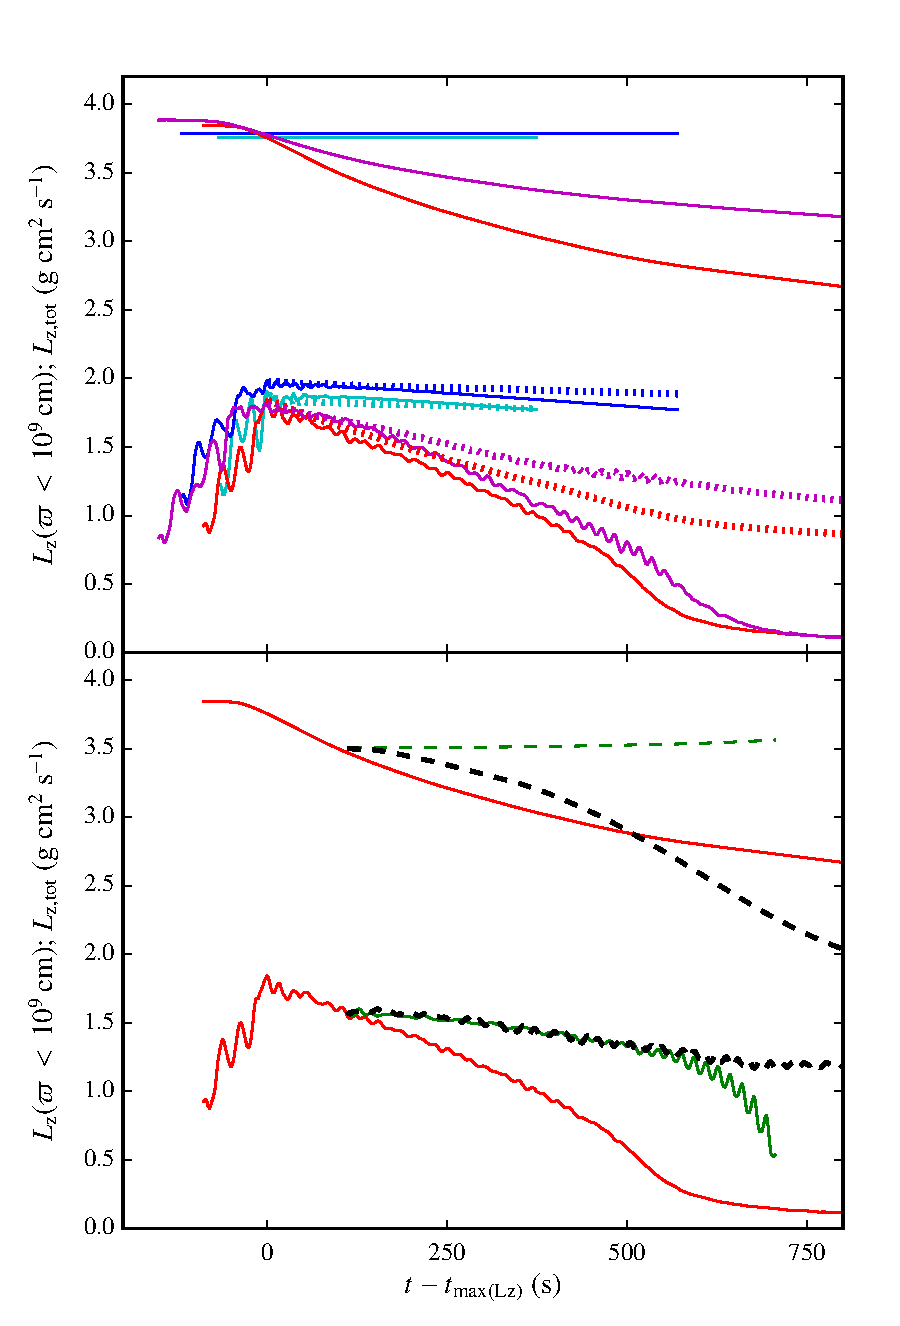
\includegraphics[angle=0,width=0.6\columnwidth]{chapter3_zhu+u/figures/lz_development.pdf}
\caption{Evolution of total $z$-axis angular momentum \Lztot\ (top cluster of lines in each panel) and that within a cylinder of radius $\varpi = 10^9\,\mrm{cm}$, \Lzinner\ (bottom cluster), for various simulations in 2013-2014, before \arepo\ was updated to better conserve angular momentum.  All curves are shifted in time by \tlm, the time in each simulation at which \Lzinner\ achieved its maximum value, to synchronize the start of post-merger evolution.  In the top panel, red and magenta lines represent the low and standard-resolution \arepo\ simulations, respectively, while the cyan and blue ones represents low and standard-resolution \gasoline\ ones, respectively.  Dotted lines represent angular momentum balance $\Lbal(\winnercyl)$, which should be flat in the absence of spurious angular momentum losses.  (Slightly different initial amounts of total angular momentum between \arepo\ and \gasoline\ runs are due to inconsistencies in their initial conditions that have subsequently been eliminated.)  In the bottom panel, the red line is again the low-resolution \arepo\ simulation, while the green line is an \arepo\ low-resolution run where the mesh is held static after $t = 200\,\mrm{s}$.  The dashed black line is a \flash\ simulation that uses the \arepo\ low-resolution run at $t = 200\,\mrm{s}$ for initial conditions; its loss of total angular momentum is due to having outflow boundaries.}
\label{fig:c3_fix_angmo}
\end{figure}

In the top panel of Fig. \ref{fig:c3_fix_angmo}, we show the evolution of the total $z$-axis angular momentum \Lztot\ (top cluster of lines) for low-resolution ($1\times10^{28}\,\mrm{g}$ particles or cells) and standard-resolution ($2\times10^{27}\,\mrm{g}$) \gasoline\ and \arepo\ simulations.  We also show the angular momentum within a cylinder oriented along the rotational axis with radius \innercyl, \Lzinner, which represents the angular momentum within the dense core of the merger remnant.  Coalescence occurs at somewhat different times in the two codes (partly due to slight inconsistencies in their initial conditions that have subsequently been eliminated), so each simulation's curve is shifted by \tlm, the time at which \Lzinner\ achieves its maximum value (a rough proxy for the end of coalescence).  We see that, over $\sim1000\,\mrm{s}$, the \arepo\ remnant's angular momentum drops by a factor of $\sim20$ at both resolutions, behavior that is not reproduced by either \gasoline\ run.  The spiral waves generated in \arepo\ are a mechanism for transporting angular momentum (eg. \citealt{balb03}) and were initially presumed to be the cause of this remnant spin-down.  Global angular momentum in \arepo, however, is not conserved: the low-resolution run loses a \textit{third} of its angular momentum over $\sim1000\,\mrm{s}$, and the standard-resolution one about a fifth.  SPH formally conserves angular momentum, and we find the \Lztot\ for \gasoline\ varies in time by $\lesssim5\times10^{-5}$ from its mean values at either resolution.

% Arepo doesn't have a fixed resolution, and so the number of mesh generating points will increase with time.  The low-res NoVolRef run on magny starts at 255,035 and and ends at 1000 s with 6,397,501 points (remember to remove the background grid with dc.d["backgrid"] < 0.5!).  The high-res one starts at 1,275,092 points and ends with 1,607,823 points.

A moving mesh that refines in regions of high density may not properly resolve the disk of the merger remnant (which is at low-density but carries much of the remnant's angular momentum).  To better pinpoint where the angular momentum was being spuriously lost, we computed (similar to \citealt{ji+13}, their Sec. 2.2.4) the theoretically expected change in \Lz.  For a cylinder $V$ oriented along the rotational axis, this is given (via the Euler equations) by

\eqbegin
\frac{\ptl \Lz}{\ptl t} = - \oint_V \rho \varpi v_\phi v_\varpi dS + \int_V {\boldmath \varpi}\times{\bf \nabla}\Phi dV
\label{eq:c3_angmobalance}
\eqend

%\eqbegin
%\frac{\ptl L_i}{\ptl t} = - \oint_V \epsilon_{ijk} \rho x^ju^k u_l dl^l + \int_V \epsilon_{ijk} x^j F^k dV - \int_V \epsilon_{ijk} x^j \ptl^kP dV
%\label{eq:angmobalance}
%\eqend

% PROOF PRESSURE TORQUE IS ZERO (http://adama.astro.utoronto.ca/~cczhu/mergerwiki/doku.php?id=nov2013&#november_8th):
%\begin{eqnarray}
%\left(\int_V \epsilon_{ijk} x^j \partial^kP dV\right)_z &=&\int_r\int_\phi r \frac{\partial P}{\partial \phi} rdrd\phi \nonumber \\
%&=& \int_r r^2 (\int_\phi \frac{\partial P}{\partial \phi} d\phi)dr \nonumber \\
%&=& \int_r r^2 (P(2\pi) - P(0))dr \nonumber \\
%&=& 0 \nonumber
%\end{eqnarray}

\noindent where the first term encapsulates advection out of the volume (including the Reynolds stress associated with wave motion; \citealt{balb03, kratl16}) and the second term external torque -- in our case gravitational.\footnote{A third, pressure torque term also arises in general, but for a cylinder oriented along the axis of rotation it is analytically zero (and numerically negligible as well).}  Subtracting the time-integral of Eqn. \ref{eq:c3_angmobalance} (i.e. the cumulative angular momentum change $\Delta \Lz$) from the volume's angular momentum gives us the ``balance''

\eqbegin
\Lbal(t) = \Lz(t) - \Delta \Lz = \Lz(t) - \int_{t_0}^{t}\frac{\ptl \Lz}{\ptl t'}dt'.
\label{eq:c3_angmobalance2}
\eqend

\noindent In a system with perfect angular momentum conservation, $\Delta \Lz$ would account for all changes in $\Lz(t)$ and $\Lbal(t) = \Lbal(t_0)$ would be a constant.  

In Fig. \ref{fig:c3_fix_angmo}, we show using dashed lines the balance for the cylinder of $\varpi = 10^9\,\mrm{cm}$, $\Lbal(\winnercyl)$, for each of the four simulations, to check for spurious changes to the angular momentum of the merger remnant cores.  While $\Lbal(\winnercyl)$ decreases by $\sim5$\% in the \gasoline\ simulations (likely due to artificial viscosity, not included in Eqn. \ref{eq:c3_angmobalance}), the change in \Lbal\ accounts for approximately \textit{all} of the total spurious losses in \arepo\ at high resolution (compare the \Lztot\ and \Lbal\ lines), invalidating the hypothesis that it is the outer regions of the simulation spuriously losing angular momentum.  

% Arepo Lz losses determined by taking the first and last points in the balance.p files, eg. "arl_old.d["Lz"][-1,-1]/arl_old.d["Lz"][0,-1]"

We then hypothesized that low-density regions near \innercyl\ that interact with the remnant core were under-resolved. To rectify this, we performed a run which, after coalescence, included a volume refinement scheme for cells within $\varpi\,=\,10^9\,\mrm{cm}$.  This led to a dramatic increase in resolution over time, with the simulation eventually exceeding $2\times10^7$ cells.  This run loses $\sim5$\% of \Lztot\ in $\sim500\,\mrm{s}$, but $\sim30$\% of the change in \Lzinner\ over the same timespan is still spurious, meaning losses would only be rendered negligible at impractically high resolutions.

% From Phil Chang: "The grid that I used was an outer grid of 256^3 in a box whose size was 1.6e5 km on the side (\Delta x = 624 km).  Two refined grids were deployed.  First level of refinement was at a scale < 50000 km from the center and a factor of 4 enhancement (Delta x = 156 km).  Second level was at a scale of 30000 km from the center and was a factor of 2 enhancement in resolution (Delta x = 78 km).  The second level basically covered the remnant. Effective resolution was 2048^3.  Gravity was solved using the multipole method with an lmax=50 (check was used with a multigrid method and a multipole with lmax=200 and no real differences were found). Solver was unsplit with a HLLC Riemann solver for HD and HLLD for MHD."

%$\sim10^7\,\mrm{cm}$

%(chosen to be $\sim2$ orbital periods after coalescence)

We finally turned to simulating post-merger evolution in other codes.  In the bottom panel of Fig. \ref{fig:c3_fix_angmo}, we show our simulation in the Eulerian code \flash\ (\citealt{fryx+00, dube+09}) that uses the low-resolution \arepo\ run at $t = 200\,\mrm{s}$ for initial conditions.  In \flash, we used a 3D Cartesian grid $1.6\times10^{10}\,\mrm{cm}$ to a side, with multiple levels of fixed-mesh refinement centered on the merger remnant so that its core is resolved with cells $7.8\times10^6\,\mrm{cm}$ to a side (comparable to the low-resolution \arepo\ run).  Gravity was solved using a multipole solver with $l_\mrm{max} = 50$, and fluxes propagated with the HLLC (Harten-Lax-van Leer -- Contact) Riemann solver.  We also show a low-resolution \arepo\ run where, at $t = 200\,\mrm{s}$, the mesh's velocities were forced to zero, transforming \arepo\ into a static grid code operating on an unstructured mesh.  Considering the sheer number of differences between the two simulations, they agree remarkably on the rate of change of \Lzinner\ until very late times (when mesh drift issues corrupt the \arepo\ simulation).  \Lztot\ for the \arepo-static run also changes by only $\sim1$\% over $\sim500\,\mrm{s}$.  These simulations suggested \arepo's moving mesh scheme cause spurious angular momentum loss.

%\footnote{We also attempted to transport \arepo\ simulation snapshots following coalescence into \gasoline, and vice versa.  The former showed angular momentum transport and the spiral pattern fading away within $\sim150$ s, while the latter showed the onset of Kelvin-Helmholtz instabilities at the interface between the rigidly rotating and sub-Keplerian portions of the remnant, followed by angular momentum loss.  This was the case even when the \gasoline\ initial conditions were nearly axisymmetric, and stable to hydrodynamic instability by \cite{maed+13}'s modified Solberg-H{\o}iland criterion.}

Eventually, \cite{pakm+16} found two aspects of \arepo's original hydrodynamic scheme (Sec. \ref{ssec:c3_arepo}) were responsible for making the code only \textit{first-order} convergent for non-trivial moving meshes.  First, while Eqn. \ref{eq:c3_muscl_hancock} provides second-order convergence on static meshes of arbitrary geometry, it only uses the initial state of the mesh itself, and so reduces to first-order on moving meshes.  Second, \arepo's estimate for $\phi({\bf f}_{ij})$ in Eqn. \ref{eq:c3_gauss_green} assumes that the cell centers of mass ${\bf s}_i$ -- where the value of ${\bf W}_i$ is defined -- and mesh-generating points ${\bf r}_i$ align, which is not true for elongated cells.  This first-order convergence does not inevitably cause major errors -- the galaxy formation study of \cite{marips14} is not affected, for example -- but for a rotation-dominated system being simulated over many tens of dynamical times, such as the accretion disk in \cite{pakm+16}, systematic deviations in angular momentum conservation become large.

The solution is correspondingly two-fold: first, replace Eqns. \ref{eq:c3_arepo_timeadv} and \ref{eq:c3_muscl_hancock} by a hybrid of the MUSCL and 2nd order Runge-Kutta methods:

\begin{eqnarray}
{\bf W}^\prime_i &=& {\bf W}^n_i + \Delta t \, \frac{\ptl {\bf W}}{\ptl t} \nonumber \\
{\bf r}_i^\prime &=& {\bf r}_i^n +  \Delta t \, {\bf w}_i^n \nonumber \\
{\bf Q}^{n+1}_i &=& {\bf Q}^n_i - \frac{\Delta t}{2} \, \left( \sum_j A^n_{ij} {\bf \hat{F}}_{ij}^{n} \left( {\bf W}^n \right) + \sum_j A^\prime_{ij} {\bf \hat{F}}_{ij}^{\prime} \left( {\bf W}_i^\prime \right) \right) \nonumber \\
{\bf r}_i^{n+1} &=& {\bf r}_i^\prime,
\label{eq:c3_rk2_timeevo}
\end{eqnarray}

\noindent where ${\bf w}_i$ is the velocity of the mesh-generating point (and is, as discussed above, roughly the speed of the fluid within the cell).  With this method, we first make a prediction of the cell's future primitive variables ${\bf W}^\prime$, as well as the future Voronoi mesh.  We then use both the current and predicted values to calculate an average flux (spatial extrapolation to the cell interface is implicit when calculating $\hat{F}_{ij}$) and evolve the cell.  The mesh velocities are assumed to be constant over $\Delta t$, so the predicted and true future mesh are identical.  Second, the Green-Gauss gradient estimate is replaced with a linear least-squares one, which determines slope $\left\langle \nabla \phi \right\rangle_i$ by minimizing

\eqbegin
\sum_j g_j \left(\phi_j - \phi_i - \left\langle \nabla \phi \right\rangle_i({\bf s}_j - {\bf s}_i)\right)^2,
\label{eq:c3_leastsq_grad}
\eqend

\noindent where $g_j \equiv A_{ij}/|{\bf s}_j - {\bf s}_i|^2$ is a weighting function.  This estimate gives the value that best reproduces the change in $\phi$ when traveling from cell $i$ to any of its neighbors, and relies on cell centers of mass rather than mesh generating points.  Working in concert, these Runge-Kutta and Least-Squares Fitting (RKLSF) methods make \arepo\ second-order convergent.

\begin{figure}
\centering
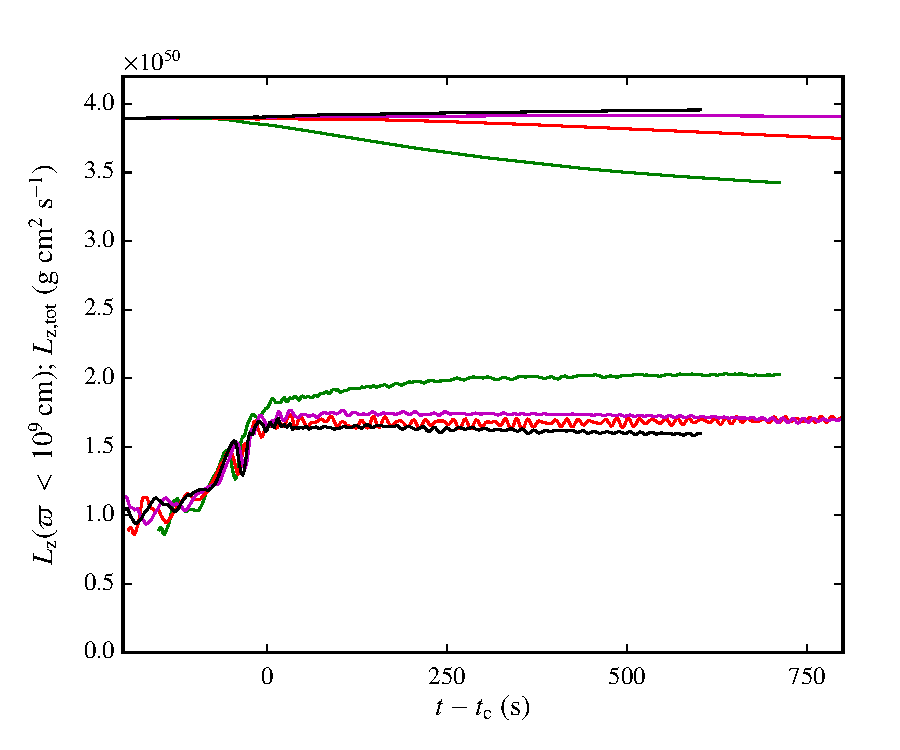
\includegraphics[angle=0,width=0.6\columnwidth]{chapter3_zhu+u/figures/lz_development2.pdf}
\caption{Evolution of total $z$-axis angular momentum \Lztot\ (top cluster of lines) and that within a cylinder of radius $\varpi = 10^9\,\mrm{cm}$, \Lzinner\ (bottom cluster) for the \arepo-RKLSF simulations.  All curves are shifted in time by \tcoal\ (rather than \tlm\ like in Fig. \ref{fig:c3_fix_angmo}), the time when average separation between donor and accretor material reaches a tenth of its initial value.  Colors indicate initial mass resolutions of $5\times10^{28}\,\mrm{g}$ (red lines), $1\times10^{28}\,\mrm{g}$ (green) $2\times10^{27}\,\mrm{g}$ (cyan) and $1\times10^{27}\,\mrm{g}$ (blue).}
\label{fig:c3_fix_angmo_nar}
\end{figure}

% green is for $5.1\times10^4$ cells, red for $2.5\times10^{5}$, magenta for $1.3\times10^{6}$ and black for $2.5\times10^6$.

In Fig. \ref{fig:c3_fix_angmo_nar}, we show the evolution of angular momentum for \arepo-RKLSF runs (from Sec. \ref{ssec:c3_restest}) at resolutions ranging from $5\times10^{28}\,\mrm{g}$ to $1\times10^{27}\,\mrm{g}$.  We immediately notice that \Lzinner\ no longer decreases with time, cementing the fact that the rapid spin-down seen in Fig. \ref{fig:c3_fix_angmo} was an artefact of spurious angular momentum loss.  Indeed, this makes it impossible to calculate \tlm\ -- we instead use ``\tcoal'' (discussed further in Sec. \ref{sec:c3_results}), the time when the average separation between donor and accretor material reaches a tenth of its value at the beginning of the simulation, to synchronize the start of post-merger evolution.  In all but the lowest-resolution run, \Lztot\ deviates by less than $\sim4$\% from its initial value, and at the highest resolution run of $1\times10^{27}\,\mrm{g}$, or $2.5\times10^6$ cells, it deviates by $\sim1.5$\% over $\sim840\,\mrm{s}$, an order of magnitude better than the $2\times10^7$ cell simulation without RKLSF.

The density and temperature profiles of the merger in the \arepo-RKLSF simulations also generally agree better with their \gasoline\ counterparts up until the end of coalescence, but the dense crescent and spiral wave that distinguish the \arepo\ merger remnant remain.
